\documentclass[border=3pt,tikz]{standalone}
\usepackage{amsmath}
\usetikzlibrary{3d} 
\usetikzlibrary{arrows}
\usetikzlibrary{shapes.geometric}
\begin{document}
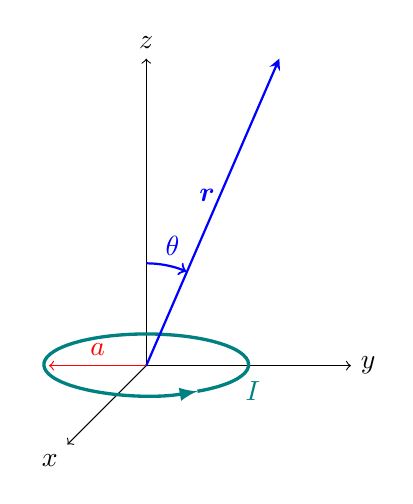
\begin{tikzpicture}[scale = 1.3, =>stealth]
    \tikzset{
        partial ellipse/.style args={#1:#2:#3}{
            insert path={+ (#1:#3) arc (#1:#2:#3)}
        }
    }
    \draw [->] (0,0) -- (xyz cs:x=2) node[right] {$y$};
    \draw [->] (0,0) -- (xyz cs:y=3) node [above] {$z$};
    \draw [->] (0,0) -- (xyz cs:z=2) node [below left] {$x$}; 
    % \draw [very thick, teal] (0.0,2) ellipse (0.5 and 2);
      
    \draw [-latex, very thick, teal] (xyz cs:x=0.5, y=-0.25) arc [start angle=300, end angle=660, x radius=1cm, y radius=0.3cm] node [xshift=20] {$I$};

 
    \draw [->, thick, blue] (xyz cs:x=0, y=1) arc [start angle=90, end angle=67, x radius=1cm, y radius=1cm] node [above,yshift=2, xshift=-5] {$\theta$};    
    \draw [blue, thick, -{stealth}] (0, 0) --node[above, xshift=-2] {$\boldsymbol{r}$} (1.3, 3);

    \draw [->, red] (0, 0) -- node[above] {$a$} (xyz cs:x=-0.95, y=0, z=0);

\end{tikzpicture}
\end{document}